\exercise{Transcritical bifurcation}{2}
We can write the normal form of the transcritical bifurcation as 
\eq{
\dot{x}=apx+bx^2
}
Find the steady states of this dynamical system, analyze their stability and draw the bifurcation diagram. 

\solution
To compute the steady states we start by demanding
\eq{
0=apx+bx^2
}
we can immediately see that $x^*=0$ is a steady state. Dividing the equation above by $x$ we find 
\eq{
0=ap+bx
}
which gives us a second steady state
\eq{
x^*=-\frac{a}{b}p
}
To determine the stability of the steady states we compute
\eq{
f_{\rm x} = ap+2bx
}
Substituting $x^*=0$, yields
\eq{
f_{\rm x} = ap
}
This shows that the steady state at 0 is stable if $ap<0$. Substituting the second steady state $x^*=-ap/b$ gives us
\eq{
f_{\rm x} = ap-2b\frac{a}{b}p = -ap
}
which shows that the second steady state is stable if $ap>0$. 

We can now draw the bifurcation diagram 
\begin{center}
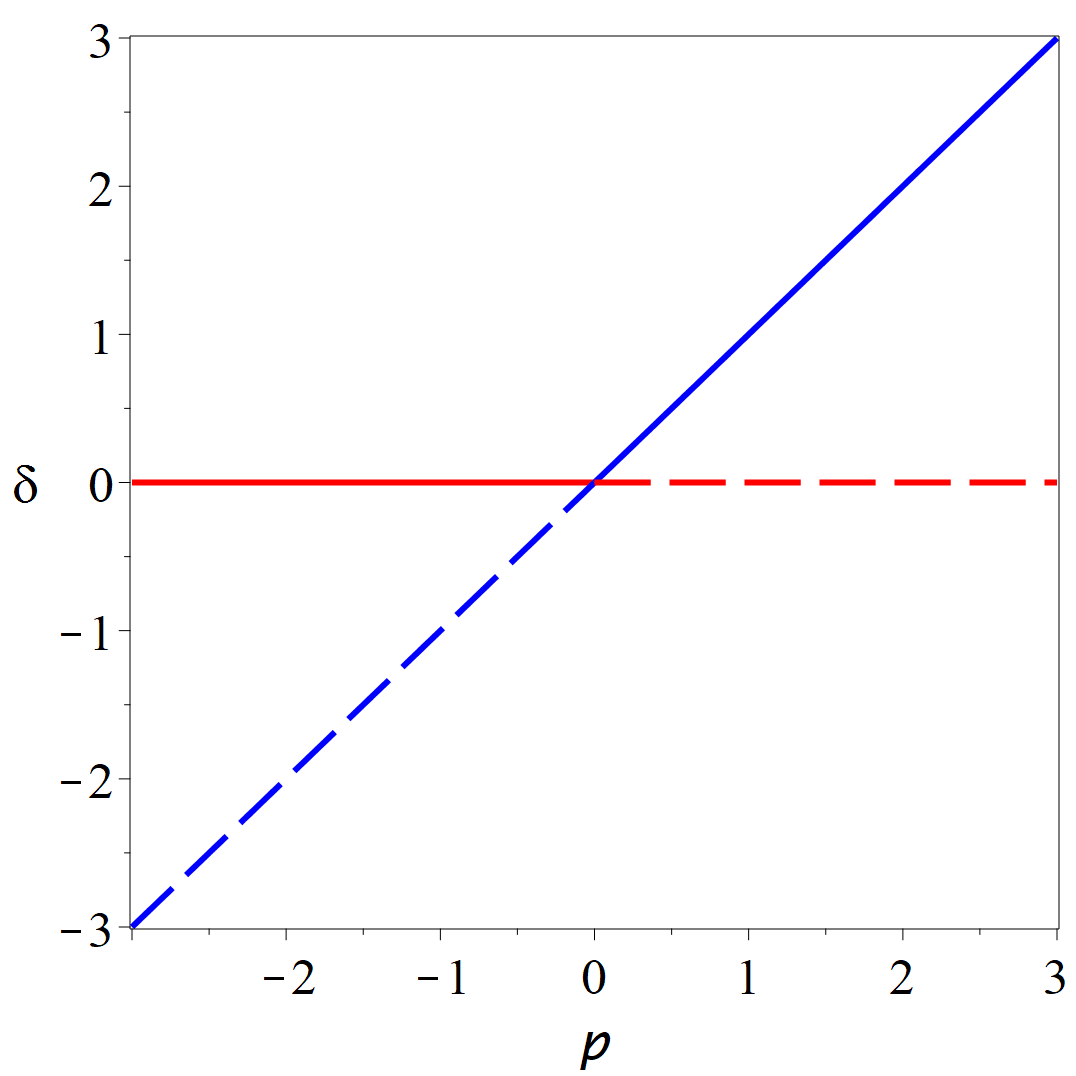
\includegraphics[width=0.6\textwidth]{Transcritical}
\end{center}
This diagram corresponds to the case $a>0$ (second steady state is stable for positive $p$) and $b>0$ (second steady state is positive for positive $p$)